\documentclass[../mathproblems.tex]{subfiles}
\graphicspath{{\subfix{../figures/}}}
\begin{document}
\chapter{AMC/AHSME}
\section{2011-}
\subsubsection*{2020 AMC 12B/8}
\textit{December 12, 2024}

How many ordered pairs of integers $(x, y)$ satisfy the equation 

\[x^{2020}+y^2=2y?\]

\textbf{Solution:}

By completing the square we get that $x^{2020}+(y-1)^2=1$.

Observe that $x=\pm 1$ or $0$ for this to work, otherwise $(y-1)^2$ will be negative which is kind of hard to do. 

Therefore, when $x=\pm 1$, we have $1+y^2=2y$, and this is equivalent when $y=1$, so we have $(-1,1)$ and $(1,1)$ as solutions.

When $x=0$, we have that $y^2=2y$, which has two solutions, when $y=0$ or when $y=2$, so we have $(0,0)$ and $(0,2)$ as solutions.

Therefore, there are $\boxed{4}$ pairs of integers that satisfy this equation.

\noindent\hrulefill

\subsubsection*{2019 AMC 12A/7} 
\textit{November 28, 2024}

Melanie computes the mean $\mu$, the median $M$, and the modes of the $365$ values that are the dates in the months of $2019$. Thus her data consist of $12$ $1\text{s}$, $12$ $2\text{s}$, . . . , $12$ $28\text{s}$, $11$ $29\text{s}$, $11$ $30\text{s}$, and $7$ $31\text{s}$. Let $d$ be the median of the modes. Which of the following statements is true?

$\textbf{(A) } \mu < d < M \qquad\textbf{(B) } M < d < \mu \qquad\textbf{(C) } d = M =\mu \qquad\textbf{(D) } d < M < \mu \qquad\textbf{(E) } d < \mu < M$

\textbf{Solution:}

I first find the mode of the numbers. The mode will be all the numbers from $1$ to $28$ since every month has those. Therefore, the median of this will be $14.5$.

The median of all the numbers will be in the $183$rd spot of all the data. There will be $12$ of each number from $1$ to $28$, and since $12(15) = 180$, we can assume that the $183$rd spot will have a $16$ there.

For the mean, if we assume that each month as $31$ days, then the mean of all these values will be $16$. However, since we counted more days than actually in the year, we assume that the mean is less than $16$.

Therefore the answer is $\boxed{\textbf{E}}$.

\noindent\hrulefill
\subsubsection*{2019 AMC 12B/7} 
\textit{November 26, 2024}

What is the sum of all real numbers $x$ for which the median of the numbers $4,6,8,17,$ and $x$ is equal to the mean of those five numbers?

\textbf{Solution:}

Ok the mean of this is simple to calculate, it is just $\frac{4+6+8+17+x}{x} = \frac{35+x}{5}$.

There are three possible medians, they are $6$, $8$, and $x$.

Case 1: median is $6$.

This only works when $x\leq 6$, so for this to work, we need $\frac{35+x}{5}=6$. This is possible when $x=-5$.

Case 2: median is $8$.

This only works when $x\geq 8$, so for this to work, we need $\frac{35+x}{5}=8$. The only value of $x$ that this works for is $x=5$, so this is not a solution.

Case 3: median is $x$.

This case is only for $6 <x <8$. We need for $\frac{35+x}{5}=x$. Simplifying this, we get $x=\frac{35}{4}$. This value is not less than $8$, so we banish this to the shadow realm!! Ok the answer is $\boxed{-5}$ btw.

\noindent\hrulefill
\subsubsection*{2018 AMC 12B/2} 
\textit{November 28, 2024}

Sam drove $96$ miles in $90$ minutes. His average speed during the first $30$ minutes was $60$ mph (miles per hour), and his average speed during the second $30$ minutes was $65$ mph. What was his average speed, in mph, during the last $30$ minutes?

\textbf{Solution:}

Using $d=rt$ we can find that in the first $30$ minutes, Sam drove $60\cdot 0.5 = 30$ miles.

In the next $30$ minutes, Sam drove $65 \cdot 0.5 = 32.5$ miles.

Therefore in the last 30 minutes, he drove $96-32.5-30=33.5$ miles. Since this is the rate for 30 minutes, simply multiply this value by two using the power of dimensional analysis in chemistry to get $\boxed{67}$ mph.

\noindent\hrulefill
\subsubsection*{2017 AMC 12B/21} 

\textit{November 27, 2024}

Last year Isabella took $7$ math tests and received $7$ different scores, each an integer between $91$ and $100$, inclusive. After each test she noticed that the average of her test scores was an integer. Her score on the seventh test was $95$. What was her score on the sixth test?

$\textbf{(A)}\ 92\qquad\textbf{(B)}\ 94\qquad\textbf{(C)}\ 96\qquad\textbf{(D)}\ 98\qquad\textbf{(E)}\ 100$

\textbf{Solution:}

The smallest possible sum and the largest possible sum that is divisible by $7$ just happens to be the lowest 7 and highest 7 numbers added together.

For example the highest possible sum is just $100+99+98+97+96+95+94 = 679 = 7(97)$, and the lowest possible sum is $91+92+93+94+95+96+97 = 658 = 7(94)$. Therefore, the only two other sums that can be $7(95)$ and $7(96)$, or $665$ and $672$.

Now we can subtract $95$ from all of them to find the sum of the first $6$ test scores.

After we subtract $95$ from all the numbers, we get $563, 570, 577, 584$. The only one of these divisible by $6$ is $570$, so we know that this is the sum of the first six test scores.

The sum of the first five test scores will have to be divisible by $5$, so note that because of this, the only numbers you can subtract from $570$ that will result in a number that can be divisible by $5$ are $95$ and $100$. $95$ cannot be subtracted from this because note the condition in the question that states that each score has to be different, so the answer is $\boxed{100}$.

\noindent\hrulefill

\subsubsection*{2016 AMC 12A/7}
\textit{December 10, 2024}

Which of these describes the graph of $x^2(x+y+1)=y^2(x+y+1)$ ?

$\textbf{(A)}\ \text{two parallel lines}\\ \textbf{(B)}\ \text{two intersecting lines}\\ \textbf{(C)}\ \text{three lines that all pass through a common point}\\ \textbf{(D)}\ \text{three lines that do not all pass through a common point}\\ \textbf{(E)}\ \text{a line and a parabola}$

\textbf{Solution:}

Case 1: $x+y+1=0$

In this case, then they are equal, so $y=-x-1$.

Case 2: $x+y+1\neq 0$

In this case, we have $x^2=y^2$, so $y=\pm x$. 

\begin{center}
    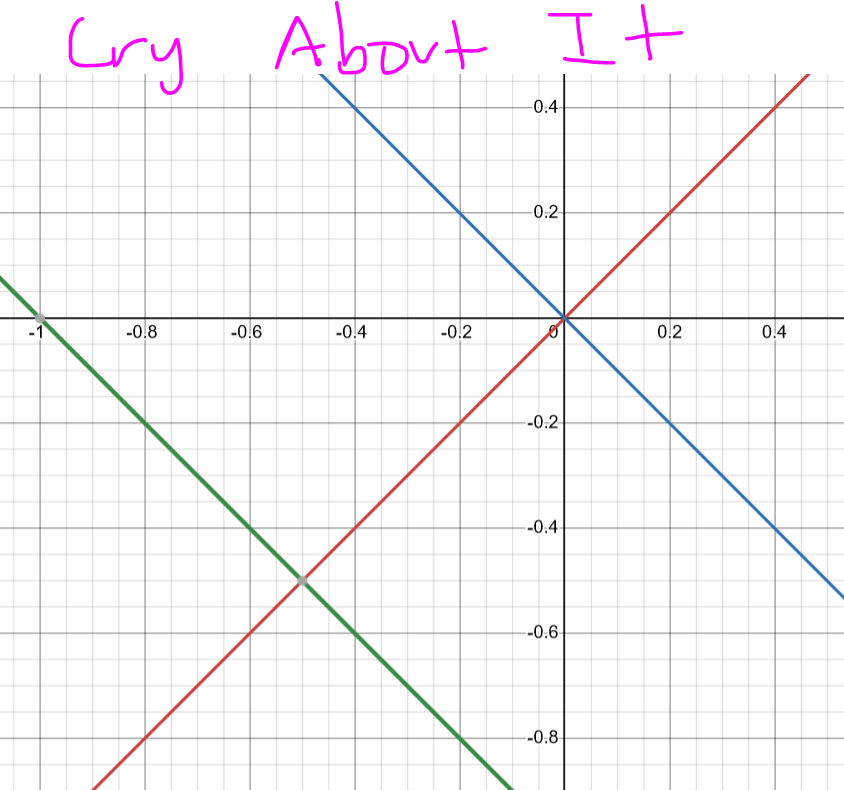
\includegraphics[width=0.4\textwidth]{vNAcilQ.png}
\end{center}

Therefore from this, we have $\boxed{\text{three lines that do not all pass through a common point}}$

\subsubsection*{2014 AMC 12A/19}
\textit{December 5, 2024}

There are exactly $N$ distinct rational numbers $k$ such that $|k|<200$ and \[5x^2+kx+12=0\] has at least one integer solution for $x$. What is $N$? 

\textbf{Solution:}

First, rearrange the equation as $5x^2+kx=-12$. Factoring out $x$ we get $x(5x+k)=-12$. Solving for $k$ we get $\frac{-12}{x}-5x$.

From here we can see that when $x$ is a positive value, and then $k$ will be negative. So, we can see that $|-5x|<200$, since the same will be for negative values of $x$.

Solving this inequality yields $-200<-5x<200$ or $40>x>-40$, where $x\neq 0$. So we can see that the values from $1$ to $39$ and $-39$ to $-1$ will be the only values that work.

Therefore $39+39=\boxed{78}$.

Note that the value $0$ will not work because the $\frac{-12}{x}$ is undefined. 

\noindent\hrulefill
\subsubsection*{2013 AMC 12A/16} 
\textit{November 21, 2024}

$A$, $B$, $C$ are three piles of rocks. The mean weight of the rocks in $A$ is $40$ pounds, the mean weight of the rocks in $B$ is $50$ pounds, the mean weight of the rocks in the combined piles $A$ and $B$ is $43$ pounds, and the mean weight of the rocks in the combined piles $A$ and $C$ is $44$ pounds. What is the greatest possible integer value for the mean in pounds of the rocks in the combined piles $B$ and $C$?

$\textbf{(A)} \ 55 \qquad \textbf{(B)} \ 56 \qquad \textbf{(C)} \ 57 \qquad \textbf{(D)} \ 58 \qquad \textbf{(E)} \ 59$

\textbf{Solution:}

We can write a few equations from the information given:
\[\frac{A}{a}=40 \qquad \frac{B}{b} = 50 \qquad \frac{A+B}{a+b} = 43 \qquad \frac{A+C}{a+c} \qquad \frac{B+C}{b+c} = x\]where $a,b,c$ are the number of rocks in piles $A,B,C$ respectively.

$A=40b$ and $B=50b$ as a result.

We can solve for $a$ in terms of $b$ now:

$A+B=43(a+b) = 43a + 43b$.

Substituting $A+B=40b+50b$, we get $40a+50b=43a+43b$.

Solving for $a$, we get $7b=3a$, and $a=\frac{7}{3}b$.

We can also solve for $C$.
\begin{align*} A+C=44a+44c\\ 40a+C = 44a+44c\\ C = 44c+4a \end{align*}
Also, we can write $C$ in terms of $b$ as well:
\begin{align*} B+C=x(b+c)\\ 50b+C=x(b+c)\\ C = xc+b(x-50) \end{align*}
Putting these equations equal to each other:
\begin{align*} 44c+4a=xc+b(x-50)\\ (44-x)c+4\left(\frac{7}{3}\right)b=(x-50)b\\ (44-x)c+\frac{28}{3}b=(x-50)b\\ (44-x)c=\left(x-50-\frac{28}{3}\right)b\\ c = \frac{\left(x-50-\frac{28}{3}\right)b}{44-x} \end{align*}
Now we can see from the answer choices that the denominator will be negative, which therefore means we need the numerator to be negative as well to result in a positive value for $c$.

$50+\frac{28}{3}$ is equal to $59\frac{1}{3}$, so the largest value $x$ that can result in the equation resulting in a positive number is $\boxed{59}$.

\noindent\hrulefill
\subsubsection*{2011 AMC 12A/18} 
\textit{December 1, 2024}

Suppose that $\left|x+y\right|+\left|x-y\right|=2$. What is the maximum possible value of $x^2-6x+y^2$?

\textbf{Solution:}

There are four cases:

$(x+y)+(x-y)$ yields $x=1$.

$-(x+y)+(x-y)$ yields $y=-1$.

$(x+y)-(x-y)$ yields $y=1$.

$-(x+y)-(x-y)$ yields $x=-1$.

This expression is maximized when the $-6x$ term is positive, and $x^2$ and $y^2$ are always going to be $1$ each, so it is maximized at $(-1,\pm 1)$, or $1^2-6(-1)+1^2=\boxed{8}$.

\noindent\hrulefill
\section{2000-2010}
\subsubsection*{2007 AMC 12A/13}
\textit{December 6, 2024}

A piece of cheese is located at $(12,10)$ in a coordinate plane. A mouse is at $(4,-2)$ and is running up the line $y=-5x+18$. At the point $(a,b)$ the mouse starts getting farther from the cheese rather than closer to it. What is $a+b$? 

\textbf{Solution:}

First we should graph the line $y=-5x+18$ and label the points.
\begin{center}
    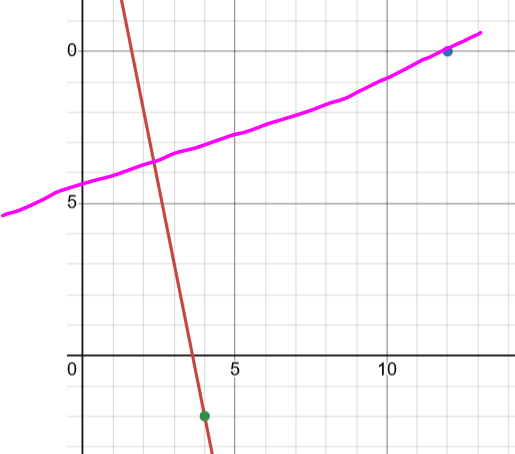
\includegraphics[width=0.4\textwidth]{GNY0Fbn.png}
\end{center}

The mouse will be closest to the cheese when it is at the foot of the perpendicular line from $(12,10)$, so we need to find the perpendicular line of $y=-5x+18$ that includes the point $(12,10)$.

From the point-slope formula we have 
\[ y-10 = \frac{1}{5}(x-12) \]

Putting this in a system with the other equation, we have 
\begin{align*}
y - 10 = \frac{1}{5}x - \frac{12}{5} \\ 
y = -5x+18
\end{align*}

When we put both of these equations equal to $y$ and equal them to each other, we have  
\begin{align*}
-5x+18 = \frac{1}{5}x + \frac{38}{5}\\
-25x + 90 = x + 38 \\
-26x = -52 \\
x = 2
\end{align*}
Plugging this back into $y=-5x+18$, we get $y=8$.

The point at which the mouse is closest to the cheese is at $(2,8)$, so $2+8 = \boxed{10}$.

\noindent\hrulefill
\subsubsection*{2006 AMC 12A/11}
\textit{December 5, 2024}

Which of the following describes the graph of the equation $(x+y)^2=x^2+y^2$?

$\mathrm{(A)}\ \text{the empty set}\qquad\mathrm{(B)}\ \text{one point}\qquad\mathrm{(C)}\ \text{two lines}\qquad\mathrm{(D)}\ \text{a circle}\qquad\mathrm{(E)}\ \text{the entire plane}$ 

\textbf{Solution:}

Simplifying the equation we have:
\begin{align*}
    (x+y)^2=x^2+y^2\\
x^2+y^2+2xy=x^2+y^2 \\
2xy=0
\end{align*}
From this we can see that $x=0$ or $y=0$, so the graphs will just be the $x$-axis and the $y$-axis which is $\boxed{\text{two lines}}$.

\noindent\hrulefill

\subsubsection*{2006 AMC 12B/8}
\textit{December 9, 2024}

The lines $ x = \frac 14y + a$ and $ y = \frac 14x + b$ intersect at the point $ (1,2)$. What is $ a + b$?

\textbf{Solution:}

Simply plug in $x$ and $y$ and we should get 
\begin{align*}
    1 = \frac{1}{2} + a \\
    2 = \frac{1}{4} + b 
\end{align*}

Adding the two equations together, we get $3=\frac{3}{4}+a+b$, so $a+b = 3-\frac{3}{4} = \boxed{\frac{9}{4}}$.

\noindent\hrulefill



\subsubsection*{2005 AMC 12B/7} 
\textit{December 4, 2024}

What is the area enclosed by the graph of $|3x|+|4y|=12$?

\textbf{Solution:}

The graph produced will be a rhombus bounded by 4 lines:

$3x+4y=12$
$3x-4y =12$
$-3x+4y=12$
$-3x-4y=12$

\begin{center}
    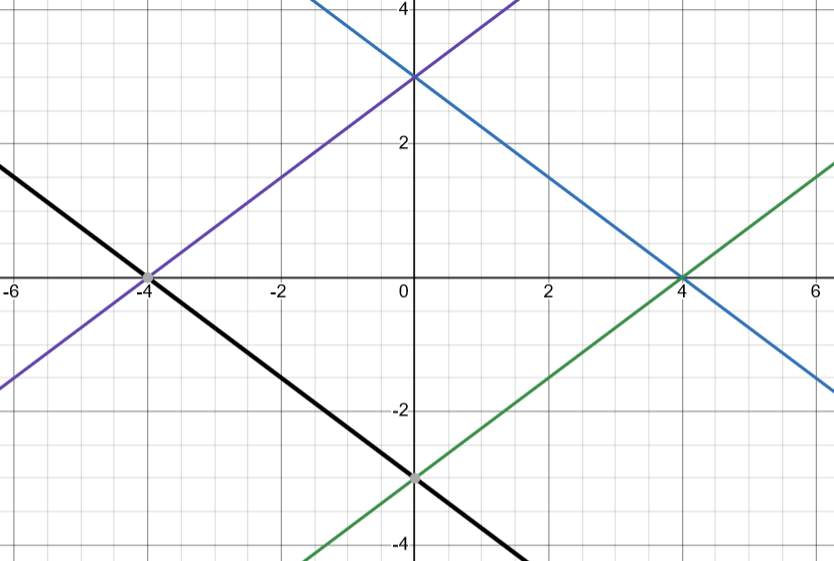
\includegraphics[width=0.4\textwidth]{f3ZKH5l.png}
\end{center}

Now the area of a rhombus is $\frac{1}{2}$ the product of the diagonals. So, $\frac{1}{2}\cdot 6 \cdot 8 = \boxed{24}$.

\noindent\hrulefill
\subsubsection*{2004 AMC 10A/4} 
\textit{November 30, 2024}

What is the value of $x$ if $|x-1|=|x-2|$?

\textbf{Solution:}

Case 1: The absolute values are less than or greater than zero.

This case does not work since $x-1\neq x-2$.

Case 2: One is positive, one is negative.

Therefore, we have $1-x=x-2$. Solving we get $x=\boxed{\frac{3}{2}}$.

\noindent\hrulefill
\subsubsection*{2000 AMC 12/5} 
\textit{December 2, 2024}

If $|x - 2| = p$, where $x < 2$, then $x - p =$

\textbf{Solution:}

Ok so $x<2$ so that means $x-2$ is negative, so $-(x-2) = p$, or $-x+2 = p$, so $x=2-p$.

Therefore $x-p = 2-p-p = \boxed{2-2p}$.

\noindent\hrulefill
\subsubsection*{2000 AMC 12/14} 
\textit{November 28, 2024}

When the mean, median, and mode of the list

\[10,2,5,2,4,2,x\]
are arranged in increasing order, they form a non-constant arithmetic progression. What is the sum of all possible real values of $x$?

\textbf{Solution:}

The list can be written as $2,2,2,4,5,10$ with $x$ somewhere.

The mode of this list is $2$ regardless of anything.

The mean of this list is $\frac{2+2+2+4+5+10+x}{7} = \frac{25+x}{7}$.

The medians can be $2$, $4$, or $x$.

If the median is $2$ and the mode is $2$, the mean has to be $2$, this is kinda erm constant.

If the median is $4$ we have $\frac{25+x}{7}$ equal to either $0$, $3$, or $6$ as the only ways to make this an arithmetic sequence.

$\frac{25+x}{7} = 0$ results in a negative number, putting this as $x$ will make the median no longer equal $4$ so it is a bad number. The same applies for $\frac{25+x}{7} = 3$. However $\frac{25+x}{7}=6$ results in a number greater than $4$, and so $x=17$.

Now the last case is when $x$ is the median. In this case, there is an arithmetic sequence of $2,x,\frac{25+x}{7}$ because the median is $x$ which is greater than $2$ and the mean of the numbers will be greater than the median.

The differences between each term have to be the same, so
\begin{align*} x-2 = \frac{25+x}{7}-x\\ 2x = \frac{25+x}{7}+\frac{14}{7}\\ 2x = \frac{39+x}{7}\\ 14x = 39+x\\ 13x = 39 \\ x = 3 \end{align*}
Since this number for $x$ is a valid median $x=3$ is also a solution.

Therefore $17+3 = \boxed{20}$.

\noindent\hrulefill
\subsubsection*{2000 AMC 12/20} 
\textit{November 24, 2024}

If $x,y,$ and $z$ are positive numbers satisfying

\[x + \frac{1}{y} = 4,\qquad y + \frac{1}{z} = 1, \qquad \text{and} \qquad z + \frac{1}{x} = \frac{7}{3}\]
Then what is the value of $xyz$ ?

\textbf{Solution:}

I noticed first that we can get $xyz$ by multiplying the equations together.

\[ \left(x+\frac{1}{y}\right) \left(y+\frac{1}{z}\right) = 4 \]\[ \left(xy + \frac{x}{z}+1+\frac{1}{yz}\right)\left(z+\frac{1}{x}\right) = \frac{28}{3} \]\[ xyz + y + x + \frac{1}{z} + z + \frac{1}{x} + \frac{1}{y} + \frac{1}{xyz} = \frac{28}{3} \]
Substituting values in, we get
\[ xyz + \frac{1}{xyz} + 4 + 1 + \frac{7}{3} = \frac{28}{3} \]\[ xyz + \frac{1}{xyz} = \frac{28}{3} - \frac{22}{3} = 2 \]
We can see that $\boxed{xyz=1}$ is a solution to this.

\noindent\hrulefill
\section{Before 2000}
\subsubsection*{1987 AHSME/15} 
\textit{November 24, 2024}

If $(x, y)$ is a solution to the system
\[ xy=6 \qquad \text{and} \qquad x^2y+xy^2+x+y=63, \]find $x^2+y^2.$

\textbf{Solution:}

Factoring the second equation, we get $xy(x+y)+x+y=63$.

Substituting in $xy$, we get $6(x+y)+x+y = 6x+6y+x+y = 7x+7y = 63$ or $x+y=9$.

Squaring both sides, we get $(x+y)^2 = x^2+y^2+2xy = 81$. Substituting in $xy$ once again, we get $x^2+y^2+2(6)=81$, so $x^2+y^2=81-12=69$.

\noindent\hrulefill

\subsubsection*{1963 AHSME/3}
\textit{December 8, 2024}

If the graphs of $2y+x+3=0$ and $3y+ax+2=0$ are to meet at right angles, the value of $a$ is:

\textbf{Solution:}

The dot product of two vectors must be $0$.

So let the two vectors be $\langle 1,2 \rangle$ and $\langle a,3\rangle$. The dot product of these two vectors, $\langle 1,2\rangle \cdot \langle a,3\rangle = (1)(a) + 2(3) = a+6$. So, when $a+6=0$, the two vectors will be perpendicular, so solving for $a$, we get $a=\boxed{-6}$.

\noindent\hrulefill



\subsubsection*{1951 AHSME/50} 
\textit{November 29, 2024}
Tom, Dick and Harry started out on a $100$-mile journey. Tom and Harry went by automobile at the rate of $25$ mph, while Dick walked at the rate of $5$ mph. After a certain distance, Harry got off and walked on at $5$ mph, while Tom went back for Dick and got him to the destination at the same time that Harry arrived. The number of hours required for the trip was:

\textbf{Solution:}

Let $x$ be the amount of miles that Harry travels on the car and $y$ be the amount that Tom backtracks to get Dick (old ah names I think).

Tom's equation will be $\frac{x}{25}+\frac{y}{25} + \left(\frac{100}{25}-\frac{x-y}{25}\right)$

Dick's equation will be $\frac{x}{5}-\frac{y}{5} + \left(\frac{100}{25}-\frac{x-y}{25}\right)$

Harry's equation will (not be so hairy) $\frac{x}{25}+\left(\frac{100}{5}-\frac{x}{5}\right)$

Note that Tom and Dick's last terms in parenthesis are the same because they will be traveling the same distance at this point in time.

Since all these equations give the time that it takes for each of these members to get to the destination, we can set them all equal to each other :-D

Aight so
\begin{align*} \frac{x+y+100-x+y}{25}=\frac{5x-5y+100-x+y}{25}=\frac{x+500-5x}{25}\\ 2y+100=4x-4y+100=500-4x \end{align*}We can solve for $y$ in terms of $x$ now:

We have $2y+100=4x-4y+100$, so cancelling out the $100$ and adding the respective terms to both sides, we get $6y=4x$ or $y=\frac{2}{3}x$.

Now substituting this value for $y$ back in to the $2y+100=500-4x$, we get that $\frac{4}{3}x+100=500-4x$. So after doing some calculations (i hate calculations), we get $x=75$.

Plugging this value for $x$ back into $y=\frac{2}{3}x$, we get $y=50$.

Now since we have both values of $x$ and $y$, we can now plug it back to one of the original equations we defined. Since Harry's little equation looks the last harriest, I plug it back into this.

$\frac{75}{25}+\frac{100-75}{5}=3+5 = \boxed{8}$

\noindent\hrulefill

\end{document}